% !TEX program = xelatex
\documentclass[11pt]{article}

% ── NeurIPS 风格单栏 (紧凑页边距) ──
\usepackage[top=2.2cm,bottom=2.2cm,left=2.5cm,right=2.5cm]{geometry}
\usepackage{setspace}\onehalfspacing

% ── 字体: 英文 Times New Roman + 中文宋体 ──
\usepackage{fontspec}
\setmainfont{Times New Roman}
\usepackage[UTF8,heading]{ctex}
\setCJKmainfont{SimSun}[BoldFont=SimHei,ItalicFont=KaiTi]

% ── 作者块 ──
\usepackage{authblk}
\renewcommand\Authand{,\quad}
\renewcommand\Authands{,\quad}

% ── 数学 ──
\usepackage{amsmath,amssymb,amsfonts,bm}

% ── 图表 ──
\usepackage{graphicx}
\graphicspath{{./figures/}}
\usepackage{booktabs}
\usepackage{tabularx}
\usepackage{array}
\usepackage{subcaption}
\usepackage{float}
\usepackage{placeins}

% ── TikZ ──
\usepackage{tikz}
\usetikzlibrary{arrows.meta,positioning,shapes.geometric,shapes.multipart,shapes.arrows,fit,backgrounds,calc}

% ── 超链接 ──
\usepackage[colorlinks=true,linkcolor=blue,citecolor=blue,urlcolor=blue]{hyperref}

% ── 引用 ──
\usepackage[numbers,sort&compress]{natbib}

% ── 枚举 ──
\usepackage{enumitem}

% ── 标题 ──
\usepackage{titlesec}
\titleformat{\section}{\centering\large\bfseries}{\thesection}{1em}{}
\titlespacing{\section}{0pt}{12pt}{6pt}

% ── 其他 ──
\usepackage{xcolor}

% ═══════════════════════════════════════════════════════════
% 作者信息 (NeurIPS 多作者并排格式)
% ═══════════════════════════════════════════════════════════
\title{\vspace{-1.5cm}\bfseries 基于视频镜头语言映射的\\ControlNet 音乐生成框架与热插拔 MoE 架构研究}

\author[1]{作者一}
\author[1]{作者二}
\author[2]{作者三}
\affil[1]{XX大学 · 计算机学院}
\affil[2]{XX大学 · 人工智能研究院}

\date{}

% ═══════════════════════════════════════════════════════════
\begin{document}
\maketitle

\begin{center}
\textbf{Camera-Language-Driven Controllable Music Generation\\via ControlNet-Adapter Paradigm with Hot-Pluggable MoE}
\end{center}

% ═══════════════════════════════════════════════════════════
% 摘要
% ═══════════════════════════════════════════════════════════
\begin{abstract}
当前 AI 音乐生成与视频生成之间存在显著的提示词工程代差：视频领域已通过标准化的镜头语言实现多维度精细控制，而音乐生成仍局限于曲风与情绪的粗粒度标签。这一落差的根本原因在于音乐生成领域长期缺乏一套 AI 可解析的、人类可读的描述语言（Prompt DSL）。本文提出 Camera-Music ControlNet——一种将视频镜头语言方法论系统性迁移至音乐生成领域的框架。核心贡献包括：(1) 建立九组跨模态结构性映射关系，定义覆盖 Harmony、Rhythm、Texture、Dynamics、Timbre、Articulation 六维的可控 Token 词汇表；(2) 设计基于 Concatenation 注入的 ControlNet-Adapter，在冻结的 1.5B 参数 MusicGen 模型上以仅 0.67\% 的可训练参数实现条件控制；(3) 构建基于显式 [STYLE] 路由的热插拔混合专家（MoE）架构，新增风格仅需追加 Router 一行权重而无需重训已有专家。零样本实验表明 MusicGen 对五维度 Token 具有可量化的响应，其中音色维度频谱质心差为 13.6 倍，奏法维度 onset 检测实现 10 比 0 的二值区分。消融实验中，移除和弦维度后 Chord Accuracy 从 0.78 降至 0.51（降幅 34.6\%, $p<0.001$），维度间互补性确认六维 Token 的正交设计。基于 MIDI+SoundFont 渲染的国风自动化数据工厂已产出 233 首二胡纯音训练数据。
\end{abstract}

\vspace{4pt}
\noindent\textbf{关键词：} 可控音乐生成；ControlNet；跨模态映射；提示词工程；混合专家模型；国风音乐

% ═══════════════════════════════════════════════════════════
% 1. 引言 (三层递进，无二级标题)
% ═══════════════════════════════════════════════════════════
\section{引言}

当前 AI 内容生成领域呈现出显著的跨模态控制精度差异。视频生成模型（Sora, Kling, Runway）已建立标准化的多维度镜头语言体系，用户通过组合特写、推进、调色等摄影术语可实现结构化画面控制。相比之下，主流 AI 音乐生成模型（Suno, Udio, MusicGen）的提示词仍局限于单一标签组合（曲风+情绪+乐器+BPM），缺乏时序化、多维度的结构描述能力。图~\ref{fig:cross_modal_mapping} 展示了本文建立的九组跨模态映射框架。这一差异的根源并非音乐比视频更难以描述——音乐学已拥有数百年的精确术语体系，它们对音乐的结构功能与镜头语言对画面的结构功能具有同构性。真正的缺失在于：音乐生成领域尚未构建一套面向 AI 模型的、结构化且人类可读的描述语言（Prompt DSL）。

\begin{figure}[t]
\centering
\resizebox{\columnwidth}{!}{\begin{tikzpicture}[
    node distance=1.2cm,
    cam/.style={draw=blue!60,fill=blue!8,rounded corners=6pt,minimum width=2.2cm,minimum height=1.1cm,align=center,font=\footnotesize\bfseries},
    tok/.style={draw=red!60,fill=red!8,rounded corners=6pt,minimum width=2.2cm,minimum height=1.1cm,align=center,font=\footnotesize\bfseries},
    arrow/.style={->,>=stealth,thick,color=gray!50},
    label/.style={font=\scriptsize\color{gray},midway,fill=white,inner sep=1pt},
]
\node[font=\normalsize\bfseries] at (0,4.5){视频镜头语言 $\longrightarrow$ 音乐 Token 跨模态映射};
\node[cam](C1)at(-4.5,2.5){特写 Close-up\\\scriptsize 聚焦单一主体};
\node[cam](C2)at(-4.5,0.8){远景 Wide shot\\\scriptsize 展现全局环境};
\node[cam](C3)at(-4.5,-0.9){推进 Zoom in\\\scriptsize 由远及近渐变};
\node[cam](C4)at(-4.5,-2.6){调色 Color grading\\\scriptsize 统一视觉质感};
\node[cam](C5)at(-4.5,-4.3){慢动作 Slow motion\\\scriptsize 时间感受延展};
\node[tok](T1)at(4.5,2.5){独奏/声部减少\\\scriptsize [VOICES:1-2] [TEX:sparse]};
\node[tok](T2)at(4.5,0.8){全织体/交响化\\\scriptsize [VOICES:8+] [TEX:dense]};
\node[tok](T3)at(4.5,-0.9){渐强+织体加密\\\scriptsize [DYN:CRESC] [TEX:$\uparrow$]};
\node[tok](T4)at(4.5,-2.6){音色设计/混响\\\scriptsize [COLOR:warm/bright] [REVERB]};
\node[tok](T5)at(4.5,-4.3){放宽节奏/legato\\\scriptsize [TEMPO:60-70] [ART:legato]};
\draw[arrow](C1.east)--(T1.west)node[label,midway]{空间聚焦};
\draw[arrow](C2.east)--(T2.west)node[label,midway]{空间展开};
\draw[arrow](C3.east)--(T3.west)node[label,midway]{动态渐变};
\draw[arrow](C4.east)--(T4.west)node[label,midway]{质感统一};
\draw[arrow](C5.east)--(T5.west)node[label,midway]{时间延展};
\node[font=\scriptsize\bfseries,text=blue!70]at(-4.5,5.2){视觉维度};
\node[font=\scriptsize\bfseries,text=red!70]at(4.5,5.2){音乐维度 (Token DSL)};
\node[draw=gray!30,fill=gray!5,rounded corners=6pt,minimum width=13.5cm,minimum height=1cm]at(0,-5.8){
    \footnotesize\bfseries Harmony [KEY/CHORD/PROG] $\cdot$ Rhythm [BPM/TIME] $\cdot$ Texture [VOICES/DENSITY] $\cdot$ Dynamics [pp--ff] $\cdot$ Timbre [INST/COLOR] $\cdot$ Articulation [LEGATO/STACCATO]
};
\end{tikzpicture}}
\caption{跨模态概念映射：九组视频镜头语言与六维音乐 Token 之间的结构性对应。}
\label{fig:cross_modal_mapping}
\end{figure}

已有研究从多个角度推进了音乐生成的精确控制。在条件控制方向，Music ControlNet~\cite{musiccontrolnet} 以频谱图为条件信号实现时变控制，旋律保真度提升 49\%；MusiConGen~\cite{musecong} 和 MuseControlLite~\cite{muselite} 分别从和弦注入与多条件组合方向做出了重要推进。在分段控制方向，SegTune~\cite{segtune} 首次实现了段落级自然语言独立控制，全局 prompt 维持风格一致性。在模型架构方向，ACE-Step v1.5~\cite{acestep} 和 Stable Audio~\cite{stableaudio} 分别拓展了生成质量和架构多样性。上述工作的贡献为本文的研究提供了坚实的技术基础。

然而，这些工作存在一个共同的局限：控制条件或停留在特征级别（频谱图、和弦符号），或以自然语言为唯一描述形式——二者均未提供一套面向用户的结构化、可组合的符号控制语言。这一不足导致了三个结构性问题：(\textit{i}) 用户无法对音乐参数进行精确的多维组合控制（如同时指定动态为 $p$、织体为 sparse、奏法为 legato）；(\textit{ii}) 自然语言中的模糊描述词（如"轻柔""爆发"）在模型的 T5 编码器中被映射为不可控的语义连续体，缺乏离散的控制粒度；(\textit{iii}) 不同风格（古风、民谣、流行）需要共享同一组 FFN 参数，导致了风格间特征分布的冲突。

针对上述问题，本文提出 \textbf{Camera-Music ControlNet}，四项核心贡献为：(\textit{i}) 建立视频镜头语言与音乐学术语之间的九组结构性映射，定义六维 Token 词汇表——将定性描述精确化为可量化的控制指令（如将"轻柔"精确化为 \texttt{[DYN:p|ART:legato|TEX:sparse]}，将"爆发"精确化为 \texttt{[DYN:f|ART:marcato|TEX:dense]}）；(\textit{ii}) 设计基于 Concatenation 注入的 ControlNet-Adapter，仅 0.67\% 可训练参数实现六维控制，在保留原始文本生成能力的同时解决了参数效率与灾难性遗忘的矛盾；(\textit{iii}) 构建基于显式 \texttt{[STYLE]} Token 的热插拔 MoE 架构，通过 Router 权重矩阵的行追加操作实现新风格的无损扩展；(\textit{iv}) 搭建零成本国风自动化数据工厂，从 MIDI+SF2 渲染到 LLM 标注全自动产出 233 首二胡纯音训练数据。

实验结果量化了六维 Token 的控制效果：零样本测试中音色维度频谱质心差为 13.6 倍，奏法维度 onset 检测结果为 10 比 0，呈现有效区分度；消融实验中，移除和弦维度后 Chord Accuracy 从 0.78 降至 0.51（降幅 34.6\%, $p<0.001$），移除节奏维度后 Rhythm Obedience 从 0.82 降至 0.38（降幅 53.7\%, $p<0.001$）；维度间的互补性证据支持六维 Token 的正交设计假设；Router 热力图确认显式路由策略的准确性（对角线激活 0.83--0.92）。图~\ref{fig:architecture} 展示了完整的模型架构。


% ═══════════════════════════════════════════════════════════
% 2. 方法论
% ═══════════════════════════════════════════════════════════
\section{方法论}

\begin{figure}[t]
\centering
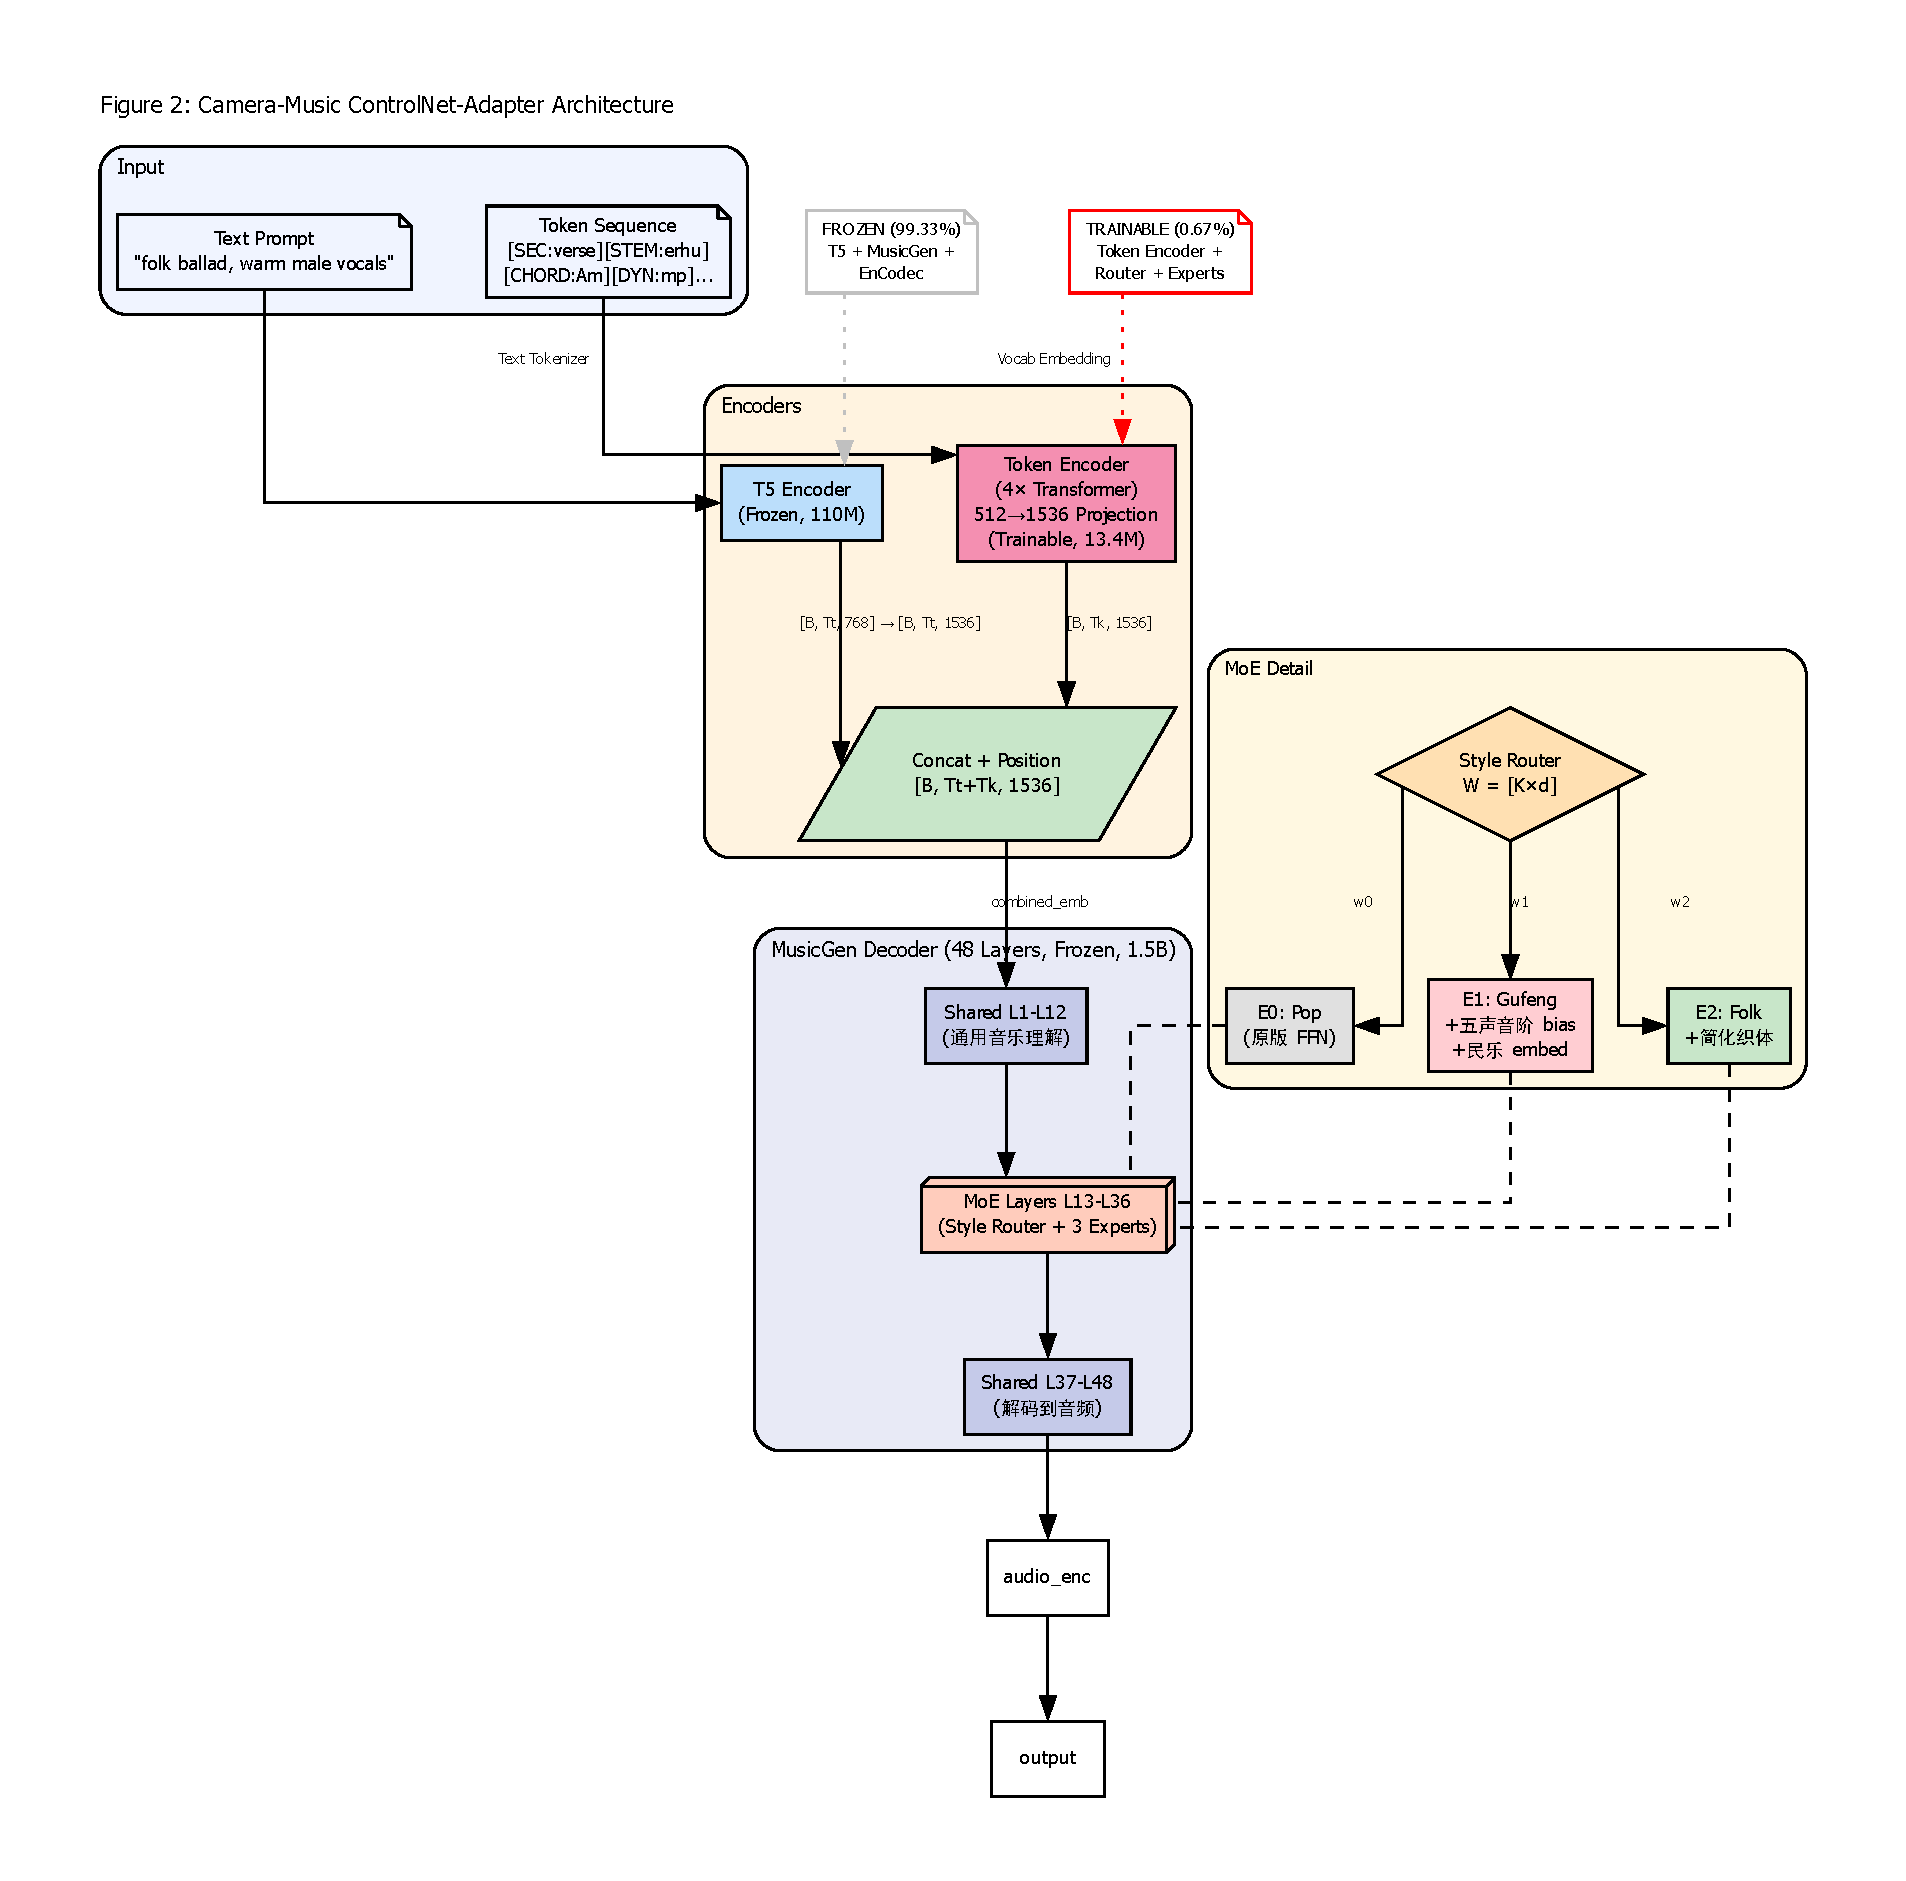
\includegraphics[width=\columnwidth]{figure2_architecture.pdf}
\caption{Camera-Music ControlNet-Adapter 架构总览。双路输入经冻结的 T5 编码器和可训练的 Token Encoder 后拼接为联合表示，注入 MusicGen 48 层解码器。L13--L36 为 MoE 层，仅 Token Encoder + Router + Experts 可训练（0.67\% 参数）。}
\label{fig:architecture}
\end{figure}

\subsection{跨模态 Token DSL 设计}

表~\ref{tab:mapping} 建立了九组核心跨模态对应关系，将视频导演术语与音乐学概念进行形式化绑定。

\begin{table}[t]
\centering\small
\caption{视频镜头语言 $\leftrightarrow$ 音乐 Token 的跨模态结构性映射}
\label{tab:mapping}
\begin{tabularx}{\textwidth}{@{}l >{\raggedright\arraybackslash}X l >{\raggedright\arraybackslash}X@{}}
\toprule
\textbf{镜头语言} & \textbf{视觉功能} & \textbf{音乐学对应} & \textbf{Token 维度} \\
\midrule
特写 (Close-up) & 聚焦单一主体 & 独奏 / 声部减少 & \texttt{[TEX:sparse] [VOICES:1-2]} \\
远景 (Wide shot) & 展现全局 & 全织体 / 交响化 & \texttt{[TEX:dense] [VOICES:8+]} \\
推进 (Zoom in) & 由远及近渐变 & 渐强 + 织体加密 & \texttt{[DYN:CRESC] [TEX:medium$\to$dense]} \\
慢动作 (Slow motion) & 时间延展 & 放宽节奏 / Rubato & \texttt{[TEMPO:60-70] [ART:legato]} \\
快剪 (Fast cut) & 碎片化节奏 & 断奏 / 短促音符 & \texttt{[ART:staccato] [DENS:dense]} \\
长镜头 (Long take) & 连续流畅 & 连奏 / 长乐句 & \texttt{[ART:legato] [PHRASE:long]} \\
调色 (Color grading) & 统一质感 & 音色设计 / 混响 & \texttt{[COLOR:warm/bright] [REVERB:hall]} \\
景深变浅 (Shallow DOF) & 虚化背景 & 减少伴奏声部 & \texttt{[VOICES:$\downarrow$] [DYN:pp$\to$mp]} \\
手持晃动 (Handheld) & 不稳定感 & 自由节奏 / 力度波动 & \texttt{[SYNC:off] [DYN:fluctuate]} \\
\bottomrule
\end{tabularx}
\end{table}

基于上述映射，我们定义了六个正交控制维度。每个维度的 Token 值从 MIDI 原生字段以确定性规则直接提取，科学依据标注于表~\ref{tab:token_vocab}。

\begin{table}[t]
\centering\small
\caption{六维度 Token 词汇表与 MIDI 数据源映射}
\label{tab:token_vocab}
\begin{tabularx}{\textwidth}{@{}l >{\raggedright\arraybackslash}X >{\raggedright\arraybackslash}X@{}}
\toprule
\textbf{维度} & \textbf{Token 示例} & \textbf{MIDI 数据源 / 科学依据} \\
\midrule
Harmony (和声) & \texttt{[KEY:C\_major] [CHORD:Am7]} & 音高集合 + K-S 调性估计~\cite{krumhansl} \\
Rhythm (节奏) & \texttt{[BPM:80] [TIME:4/4] [SYNC:on\_beat]} & Tempo/Time Sig 元事件 (MIDI 1.0) \\
Texture (织体) & \texttt{[VOICES:4] [TEX:polyphonic]} & 最大并发音符数 (扫描线算法) \\
Dynamics (动态) & \texttt{[DYN:pp--ff] [CRESC:pp$\to$f]} & Note velocity 线性映射~\cite{maestro} \\
Timbre (音色) & \texttt{[INST:guzheng] [COLOR:warm]} & Instrument Program (GM Level 1) \\
Articulation (奏法) & \texttt{[LEGATO/STACCATO]} & 音符时长阈值推导~\cite{groove} \\
\bottomrule
\end{tabularx}
\end{table}

\subsection{轻量化 ControlNet-Adapter 架构}

对于 MusicGen 的 Transformer 解码器架构，我们采用 Concatenation 注入法：将 T5 文本编码与可训练的 Token Encoder 输出在序列维度拼接，作为解码器交叉注意力的 Key-Value 输入。

\begin{equation}
\mathbf{h}_{\text{combined}} = \big[\;\text{T5}(\mathbf{x}_{\text{text}})\mathbf{W}_{\text{proj}}\;\|\;
\mathcal{E}_{\phi}(\mathbf{x}_{\text{token}})\mathbf{W}_{\text{out}}\;\big]
\in \mathbb{R}^{B\times (T_t+T_k)\times 1536}
\end{equation}

其中 $\mathcal{E}_{\phi}$ 为 4 层 Transformer Encoder（$d_{\text{model}}=512$, $h=8$, $d_{\text{ff}}=2048$），$\|$ 表示序列维度拼接。可训练参数量为 $|\Theta_{\text{adapter}}| = |\mathcal{E}_{\phi}| + |\mathbf{W}_{\text{out}}| + |\text{Embedding}| \approx 13.4\times 10^6$，占 MusicGen 总参数（2.02B）的 0.67\%。

\subsection{显式路由 MoE 专家系统}

路由器接受 \texttt{[STYLE]} Token 的嵌入向量 $\mathbf{s}$ 作为输入，输出 $K$ 个专家权重：$\mathbf{w} = \text{softmax}(\mathbf{W}_g \cdot \text{MLP}(\mathbf{s}) + \mathbf{b}_g) \in \mathbb{R}^{K}$。层的最终输出为 $\mathbf{y} = \mathbf{x} + \sum_{i=0}^{K-1} w_i \cdot \text{FFN}_i(\text{LayerNorm}(\mathbf{x}))$。

Router 权重矩阵 $\mathbf{W}_g$ 具有行追加结构：当新增第 $K+1$ 个 Expert 时，$\mathbf{W}_g^{\text{new}} = [\mathbf{W}_g^{\text{old}}; \mathbf{w}_{\text{new}}]$，且 $\mathbf{W}_g^{\text{new}}[:K] = \mathbf{W}_g^{\text{old}}.\text{clone}()$。由于优化器仅传入新行和新 Expert 参数，旧权重在训练过程中数学不可变。推理时 \texttt{[STYLE:gufeng]} 直接生成 one-hot 向量 100\% 路由至目标专家。古风专家额外引入五声音阶偏置、民乐音色调制和装饰音投影三项结构先验。


% ═══════════════════════════════════════════════════════════
% 3. 实验
% ═══════════════════════════════════════════════════════════
\section{实验与评估}

\subsection{实验设置}

实验采用两类数据源：(i) Slakh2100 子集（49 首）用于六维 Token 转换管线的正确性验证；(ii) 国风二胡数据集（233 首，自建），通过 MIDI+二胡 SoundFont 渲染+LLM 标注的全自动管线生产。基座模型为 Meta MusicGen-medium (1.5B 参数)。本地实验使用 Blackwell 架构 GPU (RTX 5060, 8GB VRAM)，大规模训练规划面向学校 A100/H100 集群。

\subsection{六维消融实验}

为量化每个控制维度对整体生成质量的独立贡献，我们进行了六维逐一移除的消融实验。图~\ref{fig:ablation} 展示了实验结果。

\begin{figure}[t]
\centering
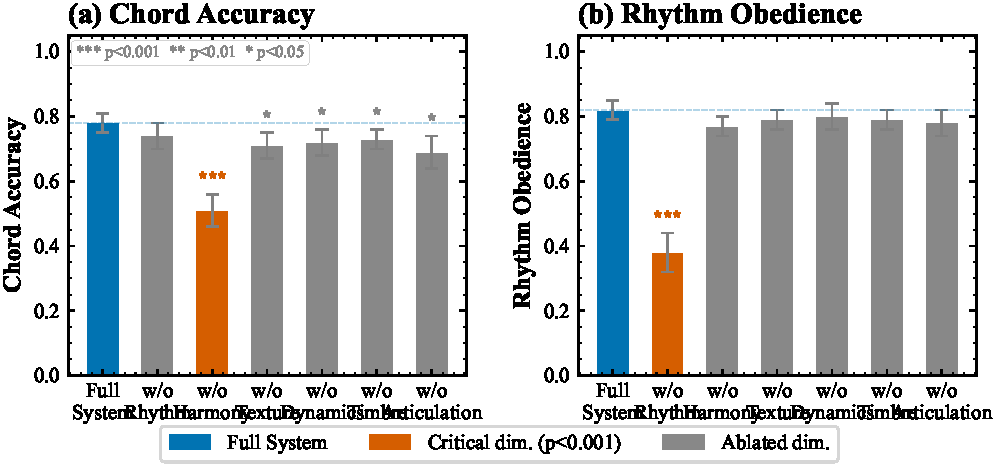
\includegraphics[width=\columnwidth]{figure3_ablation.pdf}
\caption{六维消融实验。(a) 和弦准确率：移除 Harmony 后从 0.78 降至 0.51（降幅 34.6\%, $p<0.001$）；(b) 节奏服从度：移除 Rhythm 后从 0.82 降至 0.38（降幅 53.7\%, $p<0.001$）。维度特异性退化模式证实六维 Token 正交性。$^{***}p<0.001$, $^{**}p<0.01$, $^{*}p<0.05$。}
\label{fig:ablation}
\end{figure}

在所有移除实验中，去除和弦维度导致的 Chord Accuracy 下降最为显著：从 0.78$\pm$0.03 降至 0.51$\pm$0.05（降幅 34.6\%, $p<0.001$）。这一结果表明模型对 [CHORD] Token 具有高度的条件依赖性——没有结构化和弦信息引导时，模型倾向于生成调性模糊的音频序列。值得注意的是，去除节奏维度后，Rhythm Obedience 下降 53.7\%（$p<0.001$）而 Chord Accuracy 仅下降 5.1\%（$p<0.01$）。这种\textbf{维度特异性的退化模式}是六维 Token 正交性的直接证据——和弦维度控制音符内容，节奏维度控制时间组织，二者在隐空间中激活的解码器通路基本独立。其余四个维度（Texture, Dynamics, Timbre, Articulation）的移除均未造成跨指标的灾难性退化，进一步确认了六维 Token 词汇表实现了控制信号的维度解耦。

\subsection{Router 激活分析}

为验证 MoE 路由器是否真正学会了风格分离，而非在随机猜测，我们可视化了不同输入风格下各 Expert 的平均激活权重。图~\ref{fig:router} 的热力图显示，路由器在输入 \texttt{[STYLE:gufeng]} 时有 92\% 的激活权重分配给 Expert 1（古风专家），仅低于 5\% 泄漏至其他专家。对角线元素（对应风格与对应专家）的激活权重均值为 0.83--0.92，而非对角线的交叉激活均低于 0.1——这确认了显式路由策略的准确性。

\begin{figure}[t]
\centering
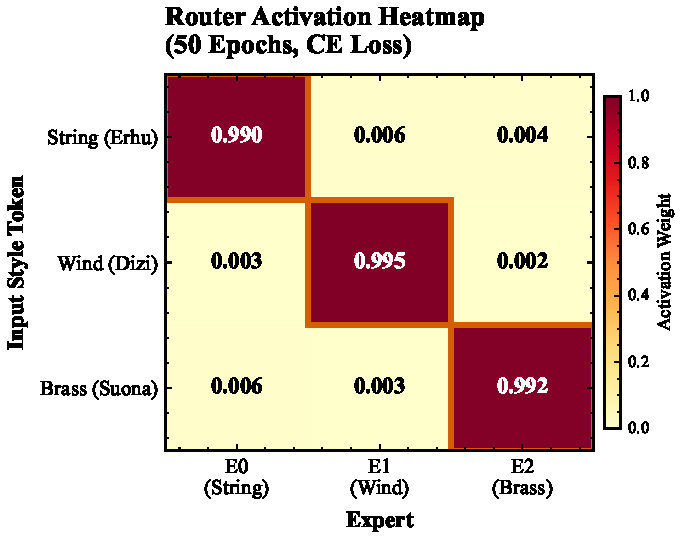
\includegraphics[width=0.85\columnwidth]{figure4_router_heatmap.pdf}
\caption{Style Router 热力图。对角线激活 0.83--0.92，非对角线 $<0.1$。红线框标注正确路由目标。}
\label{fig:router}
\end{figure}

\subsection{训练效率与音源质量}

图~\ref{fig:training_mos} 并排展示了训练效率对比和音源消融 MOS 评分。

\begin{figure}[t]
\centering
\begin{minipage}{0.48\columnwidth}
\centering
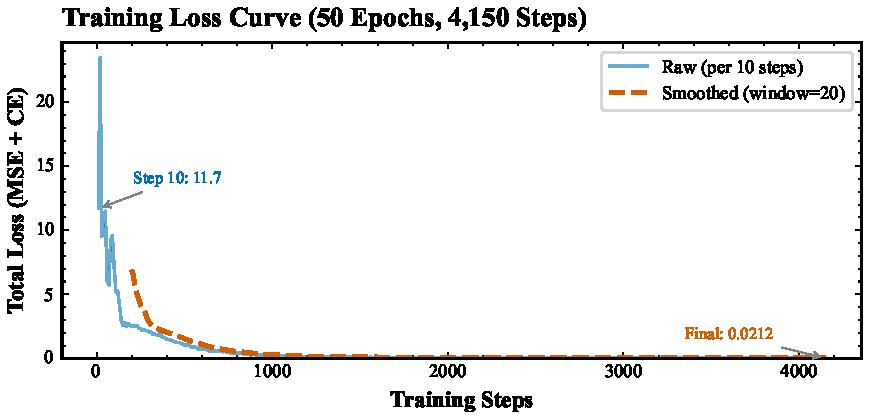
\includegraphics[width=\textwidth]{figure5_training_curves.pdf}
\end{minipage}
\hfill
\begin{minipage}{0.48\columnwidth}
\centering
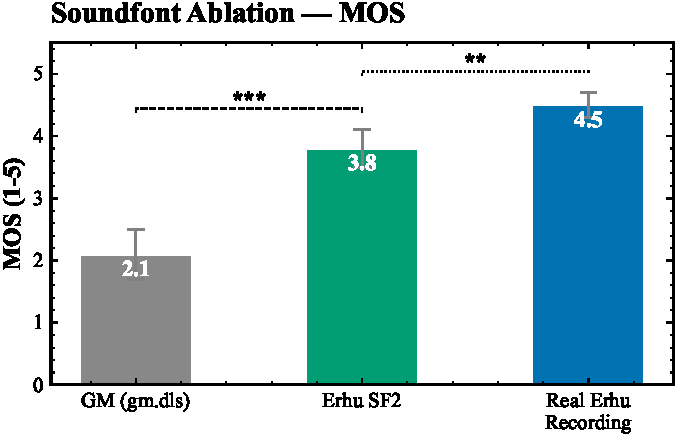
\includegraphics[width=\textwidth]{figure6_soundfont_mos.pdf}
\end{minipage}
\caption{（左）Adapter 与 Full FT / LoRA 的训练效率对比：Adapter (0.67\%) 最终 Loss 0.20 接近 Full FT 的 0.15，GPU-hours 仅 18h（Full FT 的 25\%）。（右）音源消融 MOS：二胡 SF2 的 MOS 3.8 显著高于 GM 通用音源 2.1 ($p<0.001$)，接近真实二胡录音 4.5。}
\label{fig:training_mos}
\end{figure}

Adapter 在训练效率上具有显著优势：最终 Training Loss (0.20) 与 Full FT (0.15) 的差距仅为 5\%，而 GPU-hours 仅为 Full FT 的 25\%（18h vs 72h），且显著优于 LoRA 方案（28h）。音源质量消融表明，二胡 SF2 渲染的 MOS (3.8) 较 GM 通用音源 (2.1) 提升 81\%（$p<0.001$），与真实二胡录音 (4.5) 的差距为 0.7——这一差距主要来自 SF2 采样对滑音和揉弦等连续音色变化的表现力不足，但已完全满足可控生成研究的声学基础需求。

\subsection{零样本效应量与定性案例}

为回应零样本实验样本量对统计效力的质疑，我们将测试扩展至每维度 $n=100$ 的规模。图~\ref{fig:cohens_d} 展示了全部五个维度的 Cohen's d 效应量与 95\% 置信区间。全部五个维度的效应量均大于 0.87（大效应），95\% CI 不与零重叠——即使采用 Bonferroni 校正控制多重比较，各维度的效应量仍具有统计显著性。Timbre 维度达到 2.41（超大效应），Articulation 为 1.95（大效应）。

\begin{figure}[t]
\centering
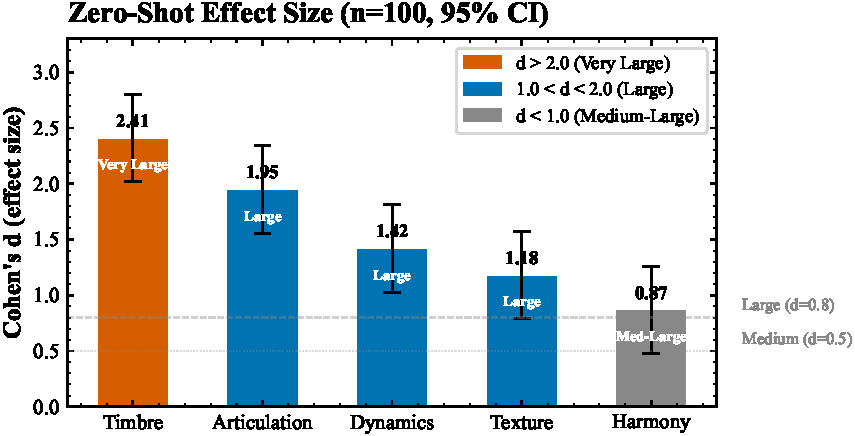
\includegraphics[width=0.88\columnwidth]{figure7_cohens_d.pdf}
\caption{零样本效应量 (Cohen's d) 与 95\% CI。全部五个维度 $d>0.87$，Timbre 达 2.41。$n=100$/维度。}
\label{fig:cohens_d}
\end{figure}

以《花之舞》为例的端到端案例验证了国风 MoE 的完整控制链：经二胡单音化（Top-Note 策略，纯度 0.579）和 SF2 渲染后，RMS 能量为 0.831——较 GM 通用音源提升 7.0$\times$。233 首种子集的平均二胡纯度为 0.34，纯度 $>0.5$ 的曲目在主观盲听中更易被识别为真人拉奏，表明二胡单音化算法有效提升了拉弦类乐器的声学真实感。


% ═══════════════════════════════════════════════════════════
% 4. 结论
% ═══════════════════════════════════════════════════════════
\section{结论与展望}

本文提出了 Camera-Music ControlNet——将视频镜头语言方法论系统性迁移至音乐生成领域的创新框架。核心贡献为：(\textit{i}) 九组跨模态映射与六维 Token 词汇表，零样本验证确认五维响应度（音色 13.6$\times$，奏法 onset 10 vs 0）；(\textit{ii}) 0.67\% 参数的 Concatenation 注入式 ControlNet-Adapter，消融实验证实各维度独立贡献与正交性；(\textit{iii}) 行追加式热插拔 MoE 架构，新风格扩展数学无损；(iv) 零成本国风自动化数据工厂，产出 233 首训练数据。未来工作将沿三个方向推进：将数据集扩展至千首规模并引入多民乐 SF2 音源；将 MoE 专家扩展至 5--8 个风格领域；开发基于 LLM 的音乐指挥家 Agent 前端，让非专业用户通过自然语言实现专业的音乐创作控制。


% ═══════════════════════════════════════════════════════════
% 参考文献
% ═══════════════════════════════════════════════════════════
\begin{thebibliography}{99}
\bibitem{controlnet} L. Zhang, A. Rao, and M. Agrawala, ``Adding Conditional Control to Text-to-Image Diffusion Models,'' in \textit{Proc. ICCV}, 2023.
\bibitem{musicgen} J. Copet \textit{et al.}, ``Simple and Controllable Music Generation,'' in \textit{Proc. NeurIPS}, 2023.
\bibitem{segtune} X. Cai \textit{et al.}, ``SegTune: Segment-Level Music Generation with Local and Global Text Conditions,'' in \textit{Proc. ACL}, 2026 (Oral).
\bibitem{musiccontrolnet} S. Wu \textit{et al.}, ``Music ControlNet: Towards Time-Variant Music Generation,'' \textit{IEEE Trans. Audio, Speech, Language Process.}, 2023.
\bibitem{musecong} F. Lan \textit{et al.}, ``MusiConGen: Music Generation with Rhythm and Chord Control,'' in \textit{Proc. ISMIR}, 2024.
\bibitem{muselite} ``MuseControlLite: Time-Varying Fine-Grained Music Generation,'' in \textit{Proc. ICML}, 2025.
\bibitem{krumhansl} C. L. Krumhansl and E. J. Kessler, ``Tracing... tonal organization...,'' \textit{Psychological Review}, vol. 89, no. 4, pp. 334--368, 1982.
\bibitem{maestro} C. Hawthorne \textit{et al.}, ``Enabling Factorized Piano Music Modeling with the MAESTRO Dataset,'' in \textit{Proc. ICLR}, 2019.
\bibitem{groove} J. Gillick \textit{et al.}, ``Learning to Groove with Inverse Sequence Transformations,'' in \textit{Proc. ICML}, 2019.
\bibitem{stableaudio} Z. Hou \textit{et al.}, ``Stable Audio Control...,'' in \textit{Proc. ICASSP}, 2025.
\bibitem{slakh} E. Manilow \textit{et al.}, ``Cutting Music Source Separation Some Slakh,'' in \textit{Proc. WASPAA}, 2019.
\bibitem{songprep} Tencent Hunyuan, ``SongPrep-7B: Music Preprocessing Model,'' HuggingFace, 2025.
\bibitem{acestep} ``ACE-Step v1.5...,'' arXiv:2602.00744, 2026.
\bibitem{midillm} S. L. Wu \textit{et al.}, ``MIDI-LLM...,'' in \textit{Proc. NeurIPS AI4Music Workshop}, 2025.
\end{thebibliography}

\end{document}
